\documentclass{article}
\usepackage{booktabs}  % 用于表格 midrule
\usepackage{multirow}  % for multirow command used in the table
\usepackage{amssymb}  % 用于打对号
%\usepackage[UTF8]{ctex} % 用于写中文
\usepackage{geometry} % 用于调整页边距
\usepackage{graphicx}  % 用于 includegraphics
\usepackage{ulem}  % 用于添加下划线
\begin{document}
\begin{table}[t]
    \centering
    \caption{Attack performance using random patterns.
    The attack performance is evaluated according to AO/SR on GOT-Val.}
    \label{table:noise}
    \begin{tabular}{@{}rcccc@{}}
    \toprule
    \multirow{2}{*}[-1pt]{\begin{tabular}[c]{@{}c@{}}Perturbations used to \\ perfrom attack \end{tabular}} & \multicolumn{2}{c}{Untargeted Attack} & \multicolumn{2}{c}{Targeted Attack}\\ \cmidrule{2-5}
                                                           & AO                                      & SR                               & AO                & SR                  \\ \midrule
    Trained Perturbations                                  & 0.153                                   & 0.123                            & 0.840             & 0.890               \\
    Similar Pattern                                         & 0.736                                   & 0.871                            & 0.153             & 0.118               \\
    Gaussian Noise                                         & 0.740                                   & 0.875                            & 0.144             & 0.101               \\ \bottomrule        
    \end{tabular}
  \end{table}
\begin{figure}[t]
    \centering
    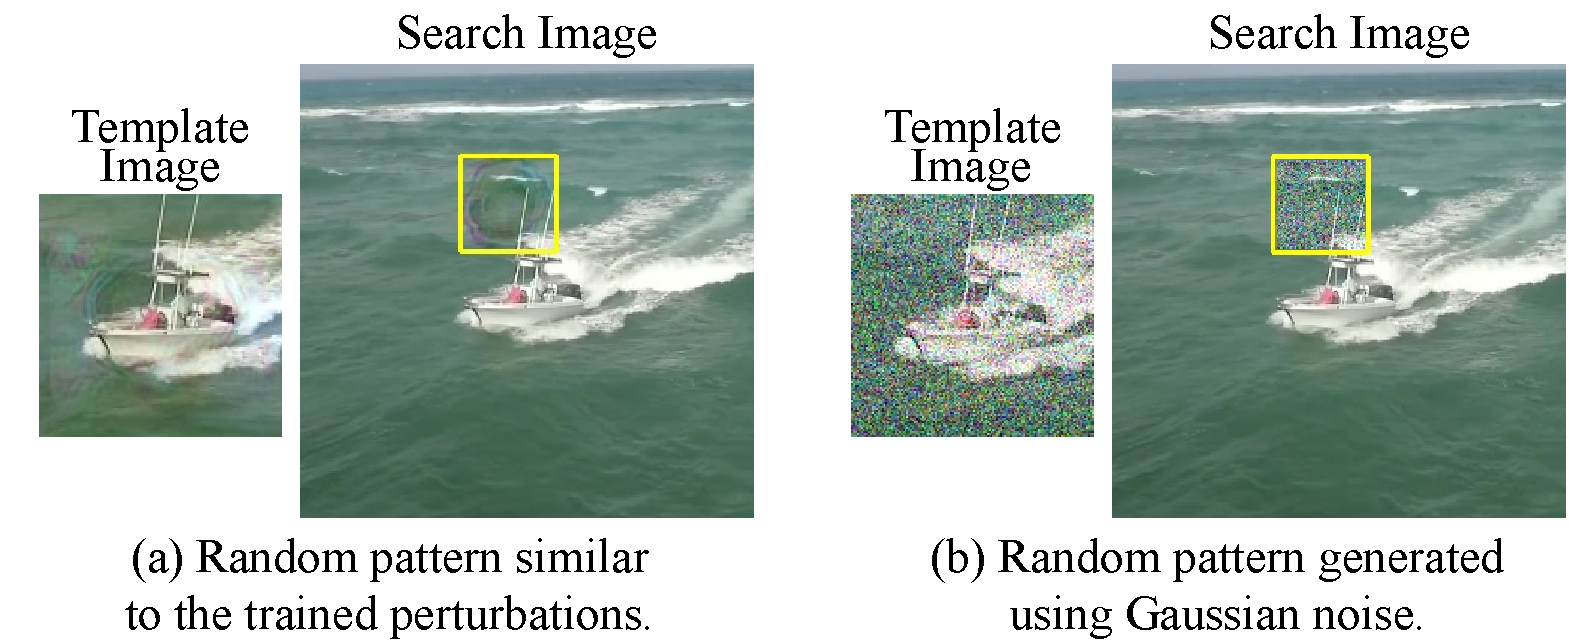
\includegraphics[width=0.8\textwidth]{random_gaussian.pdf}
    \caption{Visualization of random patterns.}
    \label{fig:random}
\end{figure}
\uline{\textit{Ablation Study: Attack performance of random patterns} To illustrate the effectiveness of the proposed method, we add random patterns on the template and search regions. 
Specifically, we design two kinds of random patterns: (1) the random pattern similar to the trained perturbations, and (2) the random pattern generated using zero-mean Gaussian noise with standard deviation 50.0.
We replace the trained perturbations with the random random pattern to attack SiamFC++\_GoogleNet. The experiment is performed on GOT-Val.
As shown in Table \ref{table:noise}, random patterns cannot effectively attack the tracker.
}
\end{document}